\subsection{图片信息增强式神经机器翻译}
% 这类方法特点不是为了解决语料中自带问题,例如歧义词,而是为了解决模型在训练过程中存在的问题,算是两种不同的思路

\begin{figure}[!htbp]
    \centering
    \begin{subfigure}{0.5\textwidth}
      \centering{
      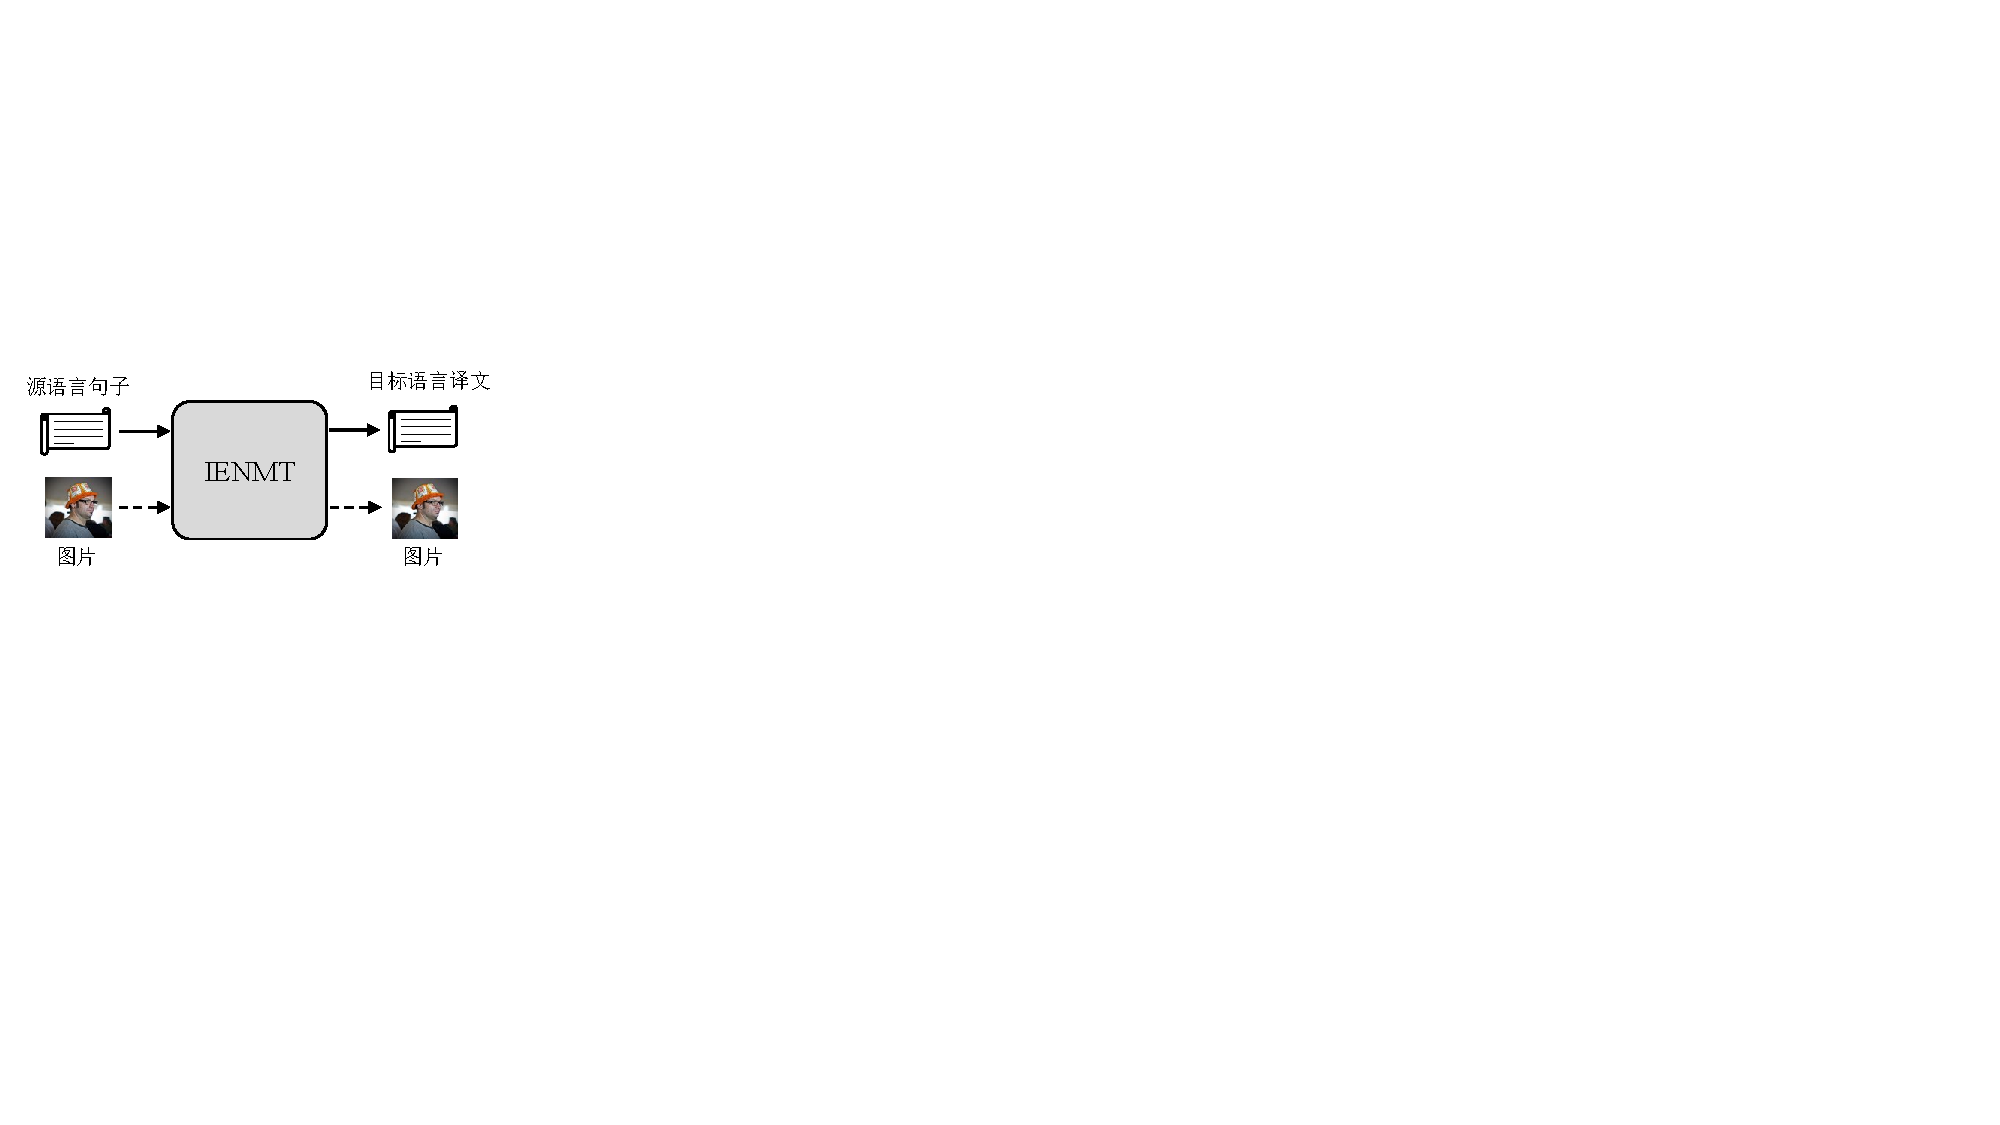
\includegraphics[width=\textwidth]{Img/fig_2_ienmt_train.pdf}
      \caption{训练阶段}
      \label{fig:2_ienmt_train}}
    \end{subfigure}%
    ~% line break
    \begin{subfigure}[b]{0.5\textwidth}
      \centering
      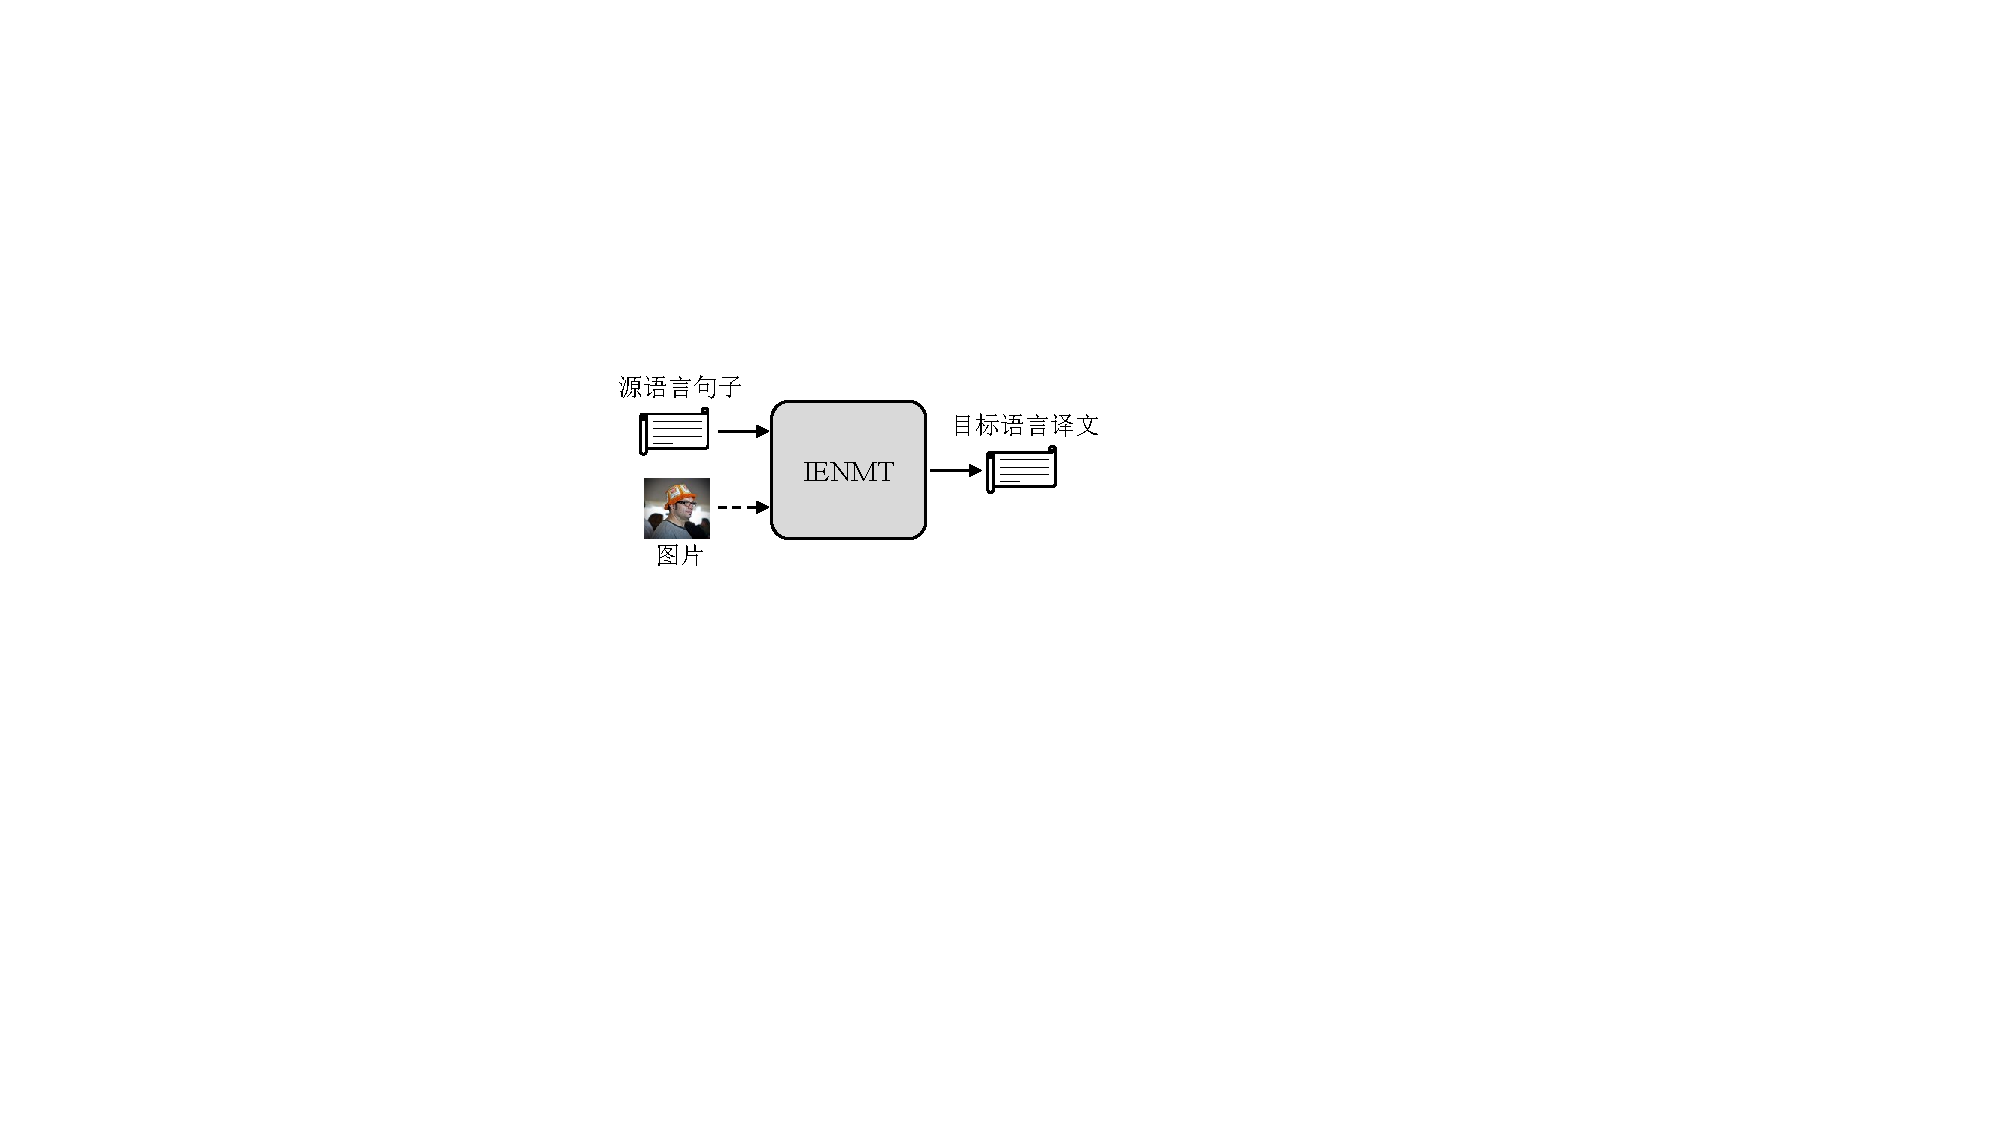
\includegraphics[width=\textwidth]{Img/fig_2_ienmt_infer.pdf}
      \caption{测试阶段}
      \label{fig:2_ienmt_infer}
    \end{subfigure}
    \bicaption{图片信息增强式神经机器翻译}{Image-enhanced neural machine translation}
    \label{fig:2_ienmt}
\end{figure}
上一节所述的图片信息辅助式神经机器翻译的主要特点是需要将图片输入到模型中,是模型利用视觉信息辅助整个翻译过程。期望通过这种方式解决待翻译文本中存在的多种病句问题,并且有大量的研究工作在这种方法范式上展开。然而,图片的作用方式不仅如此。图片信息增强式神经机器翻译(image-enhanced neural machine translation,IENMT)是一种利用特定的作用方式,将图片信息作用到模型的训练优化过程中,使神经机器翻译模型受益于这种优化方式,从而在翻译性能上得到进一步增强。图\ref{fig:2_ienmt}所示为根据目前已有的图片信息增强式神经机器翻译的相关工作总结得到的方法范式示意图。该方法的模型在训练和测试阶段的工作方式并不一致。在训练阶段,模型可以接收图片,也可以生成图片。不同的图片作用方式均有可能使模型受益。在测试阶段,模型可以是一个纯文本神经机器翻译模型,也可以融合图片信息。其工作方式主要取决于对优化过程的设计。

文献\cite{54_DBLP:journals/mt/NakayamaN17,68_DBLP:journals/corr/KirosSZ14,115_saha-etal-2016-correlational}在训练阶段将图片、源语言句子以及目标语言句子映射到一个统一的表示空间。这种方式试图将图片信息作为信息支点,然后通过将源语言和目标语言映射到这个支点,使文本的表示更忠于图片信息,从而提升纯文本翻译的质量。
文献\cite{37_elliott-kadar-2017-imagination}提出了“想象力”机制。采用向量回归的方式难以得到一个统一的表示空间,因此通过文本表示“想象”一个与图片所包含的语义相近的图像特征,能够更准确的捕捉到图片中的语义。该方法将“想象力”机制与翻译通过多任务学习的方式优化一个纯文本的神经机器翻译模型,最终得到了稳定且显著的翻译质量提升。
文献\cite{56_zhou-etal-2018-visual}在“想象力”机制的基础上增加了视觉特征初始化解码器的方式,使图片信息不仅作用的模型性能的增强,还作用到翻译过程的解码辅助中。
文献\cite{116_DBLP:conf/naacl/HirasawaYMK19}则增加预测预训练词向量来增强翻译模型。
文献\cite{117_DBLP:journals/corr/abs-1910-02766}提出了图片重建的方法。与“想象力”机制不同的是,该方法应用生成对抗网络(generative adversarial network,GAN)将文本表示映射为完整的图片特征向量。这种图片生成方式进一步作用到翻译模型的优化增强中。

上述图片信息增强式神经机器翻译方法普遍利用了文本的编码表示生成目标图像的方法范式。而这种方法主要作用到模型的编码优化过程中,没有讨论是否有优化解码器的方案。本文第3章将对该问题做进一步的研究。